\chapter{A síntese: rendimento e pureza}\label{ch:g10:synthesis-yield}

A aspirina é um dos remédios mais usados no mundo. A sua história começa
com a casca do salgueiro, mascada durante muito tempo contra a dor e a
febre; no século XIX, a substância ativa da casca foi rastreada até uma
família de compostos a partir dos quais os químicos prepararam o ácido
salicílico. Agressivo demais para o estômago para ser tomado em doses
grandes, o ácido salicílico foi transformado numa substância mais suave,
o ácido acetilsalicílico: a aspirina. Hoje ela é produzida às toneladas
em reatores de aço, pela mesma reação que um laboratório escolar
consegue fazer numa tarde. Produzir uma substância é só metade do
trabalho: também é preciso separá-la de tudo o mais que há no frasco,
purificá-la, verificá-la e pesá-la para ver quanto do que era possível
foi realmente obtido.

\begin{recall}
A \omterm{def:g10:chemical-species:extraction}{extração}, a \omterm{def:g10:chemical-species:distillation}{destilação}, a \omterm{def:g10:chemical-species:tlc}{cromatografia em camada delgada} e o \omterm{def:g10:chemical-species:retention-factor}{fator de
retenção}; um sólido puro funde a uma temperatura nítida e conhecida
(\cref{ch:g10:chemical-species}). Um filtro retém um sólido e deixa
passar um líquido (\cref{ch:g3:separating-mixtures}). A \omterm{def:g10:reaction-progress-table:extent}{tabela de avanço}
dá a quantidade máxima de produto a partir do \omterm{def:g10:reaction-progress-table:limiting}{reagente limitante}
(\cref{ch:g10:reaction-progress-table}).
\end{recall}

\begin{omfigure}
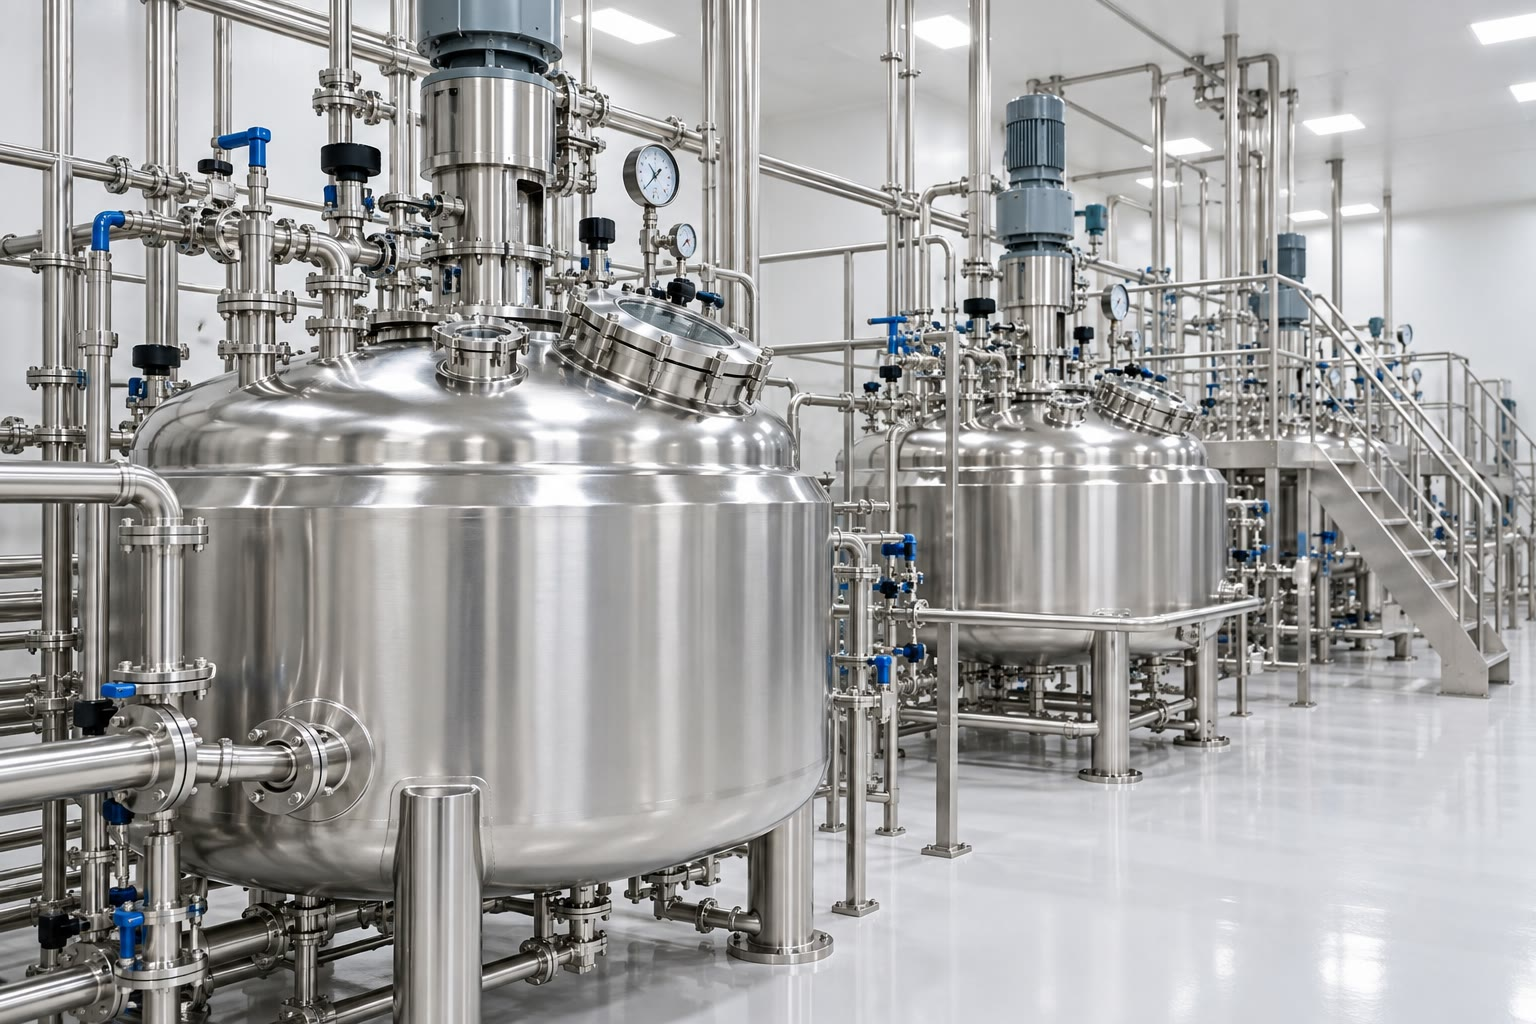
\includegraphics[width=0.55\linewidth]{images/book1/ai/g10-pharma-reactor.jpg}

{\small Reatores de aço numa indústria farmacêutica: uma \omterm{def:g10:synthesis-yield:synthesis}{síntese} de
laboratório, ampliada um milhão de vezes.}
\end{omfigure}

\section{As etapas de uma síntese}

\begin{definition}[Síntese, produto bruto]\label{def:g10:synthesis-yield:synthesis}
Uma \emph{síntese}\index{sintese@síntese} é a preparação de uma \omterm{def:g6:pure-substances-and-mixtures:species}{espécie química}
por meio de uma ou de várias \omterm{def:g7:chemical-reactions:reaction}{reações químicas}, a partir de outras
espécies. O sólido ou o líquido recuperado diretamente da \omterm{def:g6:pure-substances-and-mixtures:mixture}{mistura}
reacional, antes de qualquer purificação, é o \emph{produto
bruto}\index{produto bruto}: ele ainda contém \omterm{def:g7:chemical-reactions:reactant}{reagentes}, subprodutos e
\omterm{def:g6:solutions-and-solubility:solute}{solvente}.
\end{definition}

\begin{method}[Planejar uma síntese]\label{met:g10:synthesis-yield:plan}
Uma \omterm{def:g10:synthesis-yield:synthesis}{síntese} é feita em quatro etapas:
\begin{enumerate}
  \item \textbf{Reação}: \omterm{def:g2:mixing-and-dissolving:mix}{misturar} os \omterm{def:g7:chemical-reactions:reactant}{reagentes} nas quantidades certas,
        muitas vezes com um deles em excesso, e aquecer se necessário.
  \item \textbf{Isolamento}: separar o \omterm{def:g10:synthesis-yield:synthesis}{produto bruto} da \omterm{def:g6:pure-substances-and-mixtures:mixture}{mistura}
        reacional (\omterm{def:g3:separating-mixtures:filter}{filtração}, \omterm{def:g10:chemical-species:extraction}{extração}).
  \item \textbf{Purificação}: retirar as impurezas do \omterm{def:g10:synthesis-yield:synthesis}{produto bruto}
        (\omterm{def:g10:synthesis-yield:recrystallisation}{recristalização} para um sólido, \omterm{def:g10:chemical-species:distillation}{destilação} para um líquido).
  \item \textbf{Análise}: verificar a identidade e a pureza do produto
        (ponto de fusão, cromatografia), depois pesá-lo e calcular o
        \omterm{def:g10:synthesis-yield:yield}{rendimento}.
\end{enumerate}
\end{method}

\begin{example}[Produzir a aspirina]\label{ex:g10:synthesis-yield:aspirin}
O ácido salicílico reage com o anidrido etanoico (também chamado
anidrido acético) e dá a aspirina e o ácido etanoico:
\[
  \ce{C7H6O3 + C4H6O3 -> C9H8O4 + C2H4O2}
\]
\[
  \text{ácido salicílico} + \text{anidrido etanoico} \longrightarrow
  \text{aspirina} + \text{ácido etanoico}.
\]
O anidrido é colocado em excesso, para que todo o ácido salicílico
reaja; o ácido etanoico formado é um subproduto.
\end{example}

\begin{omfigure}
\setchemfig{atom sep=1.7em}
\begin{tabular}{@{}c@{\enspace}c@{\enspace}c@{\enspace}c@{\enspace}c@{\enspace}c@{\enspace}c@{}}
\chemfig{*6(-=-(-COOH)=(-OH)-=)} & $+$ &
\chemfig{H_3C-C(=[2]O)-O-C(=[2]O)-CH_3} & $\longrightarrow$ &
\chemfig{*6(-=-(-COOH)=(-O-[:150]C(=[:90]O)-[:210]H_3C)-=)} & $+$ &
\chemfig{H_3C-C(=[2]O)-OH} \\[2pt]
\small ácido salicílico & & \small anidrido etanoico & &
\small aspirina & & \small ácido etanoico
\end{tabular}\par\medskip

{\small A produção da aspirina, em fórmulas desenhadas (cada vértice do
hexágono é um \omterm{def:g7:atoms-and-molecules:atom}{átomo} de carbono, que leva um \omterm{def:g7:atoms-and-molecules:atom}{átomo} de hidrogênio onde
nada mais está desenhado; um capítulo mais adiante explica essa
abreviação). O grupo \ce{-OH} do anel do ácido salicílico toma metade do
anidrido; a outra metade sai como ácido etanoico.}
\end{omfigure}

\section{O aquecimento sob refluxo}

\begin{definition}[Aquecimento sob refluxo]\label{def:g10:synthesis-yield:reflux}
O \emph{aquecimento sob refluxo}\index{aquecimento sob refluxo} consiste
em aquecer uma \omterm{def:g6:pure-substances-and-mixtures:mixture}{mistura} reacional num balão encimado por um condensador
vertical: os vapores sobem, esfriam no condensador, e o líquido escorre
de volta para o balão.
\end{definition}

\begin{proposition}[Por que o refluxo]\label{prop:g10:synthesis-yield:why-reflux}
O aquecimento torna a maioria das reações mais rápida; o refluxo permite
aquecer pelo tempo necessário, à temperatura de ebulição da \omterm{def:g6:pure-substances-and-mixtures:mixture}{mistura}, sem
perder nenhum \omterm{def:g7:chemical-reactions:reactant}{reagente}, produto ou \omterm{def:g6:solutions-and-solubility:solute}{solvente} na forma de vapor.
\end{proposition}

\begin{proof}
A temperatura de um líquido em ebulição não pode subir acima do seu
ponto de ebulição, e todo vapor que escapa do líquido é condensado e
devolvido: nada sai da montagem, que fica aberta no alto para que não se
acumule pressão.
\end{proof}

\begin{omfigure}
\begin{tikzpicture}[font=\small, scale=1.05]
  \pic[transform shape] at (0,0) {heatingmantle};
  \pic[transform shape] at (0,0) {rbflask={0.42}{orange!25}};
  \foreach \p in {(-0.3,0.25), (0.2,0.18), (0.45,0.4), (-0.5,0.5)}
    \fill[black!45] \p circle (0.05);
  \pic[transform shape] at (0,3.0) {condenser};
  \draw[omDef, thick, <-] (0.8,3.825) -- (1.9,3.825) node[right] {entrada de água};
  \draw[omDef, thick, ->] (0.8,5.375) -- (1.9,5.375) node[right] {saída de água};
  \draw[omProp, thick, <-] (-0.18,5.8) -- (-1.4,6.1) node[left] {alto aberto};
  \draw[omProp, thick, <-] (-0.45,1.2) -- (-2.0,1.6)
    node[left, align=right] {mistura reacional\\ e pedrinhas de ebulição};
  \draw[omProp, thick, <-] (-1.35,-0.2) -- (-2.0,-0.6)
    node[left] {manta de aquecimento};
  \draw[omThm, ->, thick] (-0.05,3.4) -- (-0.05,4.3);
  \draw[omDef, ->, thick] (0.05,4.3) -- (0.05,3.4);
  \node[omThm, anchor=east, font=\footnotesize] at (-0.45,4.6) {o vapor sobe};
  \node[omDef, anchor=west, font=\footnotesize] at (0.85,4.6) {o líquido volta};
\end{tikzpicture}

{\small \omterm{def:g10:synthesis-yield:reflux}{Aquecimento sob refluxo}. A água fria entra na camisa do
condensador por baixo e sai por cima, de modo que a camisa fica sempre
cheia.}
\end{omfigure}

\begin{remark}[Água entrando por baixo]\label{rem:g10:synthesis-yield:water}
Alimentada por cima, a água escorreria direto para baixo e deixaria a
parte de cima da camisa cheia de \omterm{def:g4:air-a-mixture-of-gases:air}{ar}; alimentada por baixo, ela tem de
encher a camisa inteira antes de poder sair.
\end{remark}

\section{Isolar e purificar}

\begin{definition}[Filtração a vácuo]\label{def:g10:synthesis-yield:vacuum-filtration}
A \emph{filtração a vácuo}\index{filtracao a vacuo@filtração a vácuo} é uma \omterm{def:g3:separating-mixtures:filter}{filtração} em
que o líquido é puxado através do papel de filtro por sucção: um funil
achatado com uma placa perfurada (um funil de Büchner) fica sobre um
kitassato ligado a uma bomba de vácuo.
\end{definition}

\begin{omfigure}
\begin{tikzpicture}[font=\small, scale=1.05]
  \pic[transform shape] (ff) at (0,0) {filterflask={0.12}{orange!20}};
  \fill[black!50] (-0.3,2.45) rectangle (0.3,2.8);
  \pic[transform shape] at (0,2.45) {buchner={black!8}};
  \draw[black!60, line width=2pt] (ff-arm) -- (2.6,2.2);
  \draw[omProp, thick, ->] (2.7,2.2) -- (3.4,2.2) node[right,
    align=left, text=black] {para a\\ bomba de vácuo};
  \draw[omProp, thick, <-] (0.7,3.8) -- (1.9,4.3) node[right, text=black]
    {cristais no papel de filtro};
  \draw[omProp, thick, <-] (-0.4,0.15) -- (-1.8,0.6) node[left, text=black]
    {filtrado};
  \draw[omProp, thick, <-] (-0.3,2.6) -- (-1.8,2.9) node[left, text=black]
    {vedação de borracha};
\end{tikzpicture}

{\small \omterm{def:g10:synthesis-yield:vacuum-filtration}{Filtração a vácuo} com um funil de Büchner: a bomba puxa o líquido
depressa e deixa o sólido quase seco.}
\end{omfigure}

\begin{definition}[Recristalização]\label{def:g10:synthesis-yield:recrystallisation}
A \emph{recristalização}\index{recristalizacao@recristalização} purifica um sólido
dissolvendo-o no menor volume possível de um \omterm{def:g6:solutions-and-solubility:solute}{solvente} quente e depois
deixando a solução esfriar: o produto, muito menos solúvel a frio,
cristaliza, enquanto as impurezas, presentes em pequenas quantidades,
continuam dissolvidas.
\end{definition}

\begin{method}[Recristalizar um sólido]\label{met:g10:synthesis-yield:recrystallise}
\begin{enumerate}
  \item Escolha um \omterm{def:g6:solutions-and-solubility:solute}{solvente} em que o produto seja muito solúvel a quente
        e pouco solúvel a frio.
  \item Acrescente o \omterm{def:g6:solutions-and-solubility:solute}{solvente} quente aos poucos ao sólido bruto, só até
        que ele se dissolva todo.
  \item Deixe a solução esfriar devagar, depois num banho de gelo:
        formam-se cristais.
  \item Recolha-os por \omterm{def:g10:synthesis-yield:vacuum-filtration}{filtração a vácuo}, lave-os com um pouco de
        \omterm{def:g6:solutions-and-solubility:solute}{solvente} gelado e seque-os.
\end{enumerate}
\end{method}


\begin{omfigure}
\begin{tikzpicture}[font=\small]
  % 1. crude solid + a little hot solvent, on a hot plate
  \pic at (0,0.3) {hotplate};
  \pic at (0,0.3) {erlenmeyer={0.18}{orange!12}};
  \foreach \p in {(-0.4,0.42),(-0.15,0.38),(0.1,0.45),(0.35,0.4),(-0.3,0.55),(0.2,0.6)}
    \fill[brown!60] \p circle (0.06);
  \node[align=center, anchor=north] at (0,-0.15) {1. sólido bruto,\\ solvente quente};
  % 2. clear hot solution
  \pic at (3,0.3) {hotplate};
  \pic at (3,0.3) {erlenmeyer={0.22}{orange!12}};
  \node[align=center, anchor=north] at (3,-0.15) {2. tudo dissolvido,\\ límpido e quente};
  % 3. ice bath: crystals
  \fill[cyan!12, draw=black!40] (5.0,0) rectangle (7.0,1.2);
  \foreach \p in {(5.2,0.9),(6.75,1.0),(5.3,0.3),(6.8,0.25)}
    \draw[black!35, fill=white] \p ++(-0.12,-0.1) rectangle ++(0.24,0.2);
  \pic at (6,0.1) {erlenmeyer={0.2}{orange!8}};
  \foreach \x/\y in {-0.45/0.18,-0.25/0.15,0/0.2,0.25/0.15,0.45/0.2,-0.1/0.3,0.15/0.32,
                     -0.35/0.32,0.35/0.33}
    \fill[white, draw=black!55] (6+\x,0.1+\y) -- ++(0.07,0.06) -- ++(0.07,-0.06)
      -- ++(-0.07,-0.06) -- cycle;
  \node[align=center, anchor=north] at (6,-0.15) {3. esfriar no gelo:\\ formam-se cristais};
  % 4. filter
  \pic at (9,0) {filterflask={0.12}{orange!12}};
  \pic at (9,2.45) {buchner={black!12}};
  \fill[black!50] (8.7,2.45) rectangle (9.3,2.8);
  \node[align=center, anchor=north] at (9,-0.15) {4. filtrar a vácuo,\\ lavar a frio, secar};
\end{tikzpicture}

{\small A \omterm{def:g10:synthesis-yield:recrystallisation}{recristalização} em quatro etapas. As impurezas continuam
dissolvidas no \omterm{def:g6:solutions-and-solubility:solute}{solvente} frio e passam para o \omterm{def:g3:separating-mixtures:filter}{filtrado}.}
\end{omfigure}

\begin{remark}[As perdas são inevitáveis]\label{rem:g10:synthesis-yield:losses}
% ledger: sol:aspirin-25, sol:aspirin-37
Mesmo frio, o \omterm{def:g6:solutions-and-solubility:solute}{solvente} mantém um pouco de produto dissolvido. A
aspirina \omterm{def:g2:mixing-and-dissolving:dissolve}{se dissolve} na água até cerca de \qty{3.3}{g/L} a
\qty{25}{\celsius}, três vezes mais a \qty{37}{\celsius}, e muito mais
quando está mais quente: cada mililitro de \omterm{def:g3:separating-mixtures:filter}{filtrado} e de água de lavagem
leva embora um pouco de aspirina. Uma \omterm{def:g10:synthesis-yield:recrystallisation}{recristalização} compra a pureza
ao preço da massa.
\end{remark}

\section{Analisar o produto}

\begin{proposition}[Dois controles de pureza]\label{prop:g10:synthesis-yield:checks}
Um sólido sintetizado é puro, dentro dos limites destes testes, quando:
\begin{itemize}
  \item ele funde de uma vez no ponto de fusão dado nas tabelas;
  \item numa placa de \omterm{def:g10:chemical-species:tlc}{cromatografia em camada delgada}, ele dá uma única
        mancha, na mesma altura que uma amostra da \omterm{def:g6:pure-substances-and-mixtures:pure-substance}{substância pura}.
\end{itemize}
\end{proposition}

\begin{proof}
Admitido: uma impureza abaixa o ponto de fusão e o espalha por uma faixa
(\cref{ch:g10:chemical-species}), e uma segunda espécie em geral
percorre uma distância diferente na placa.
\end{proof}

\begin{omfigure}
\begin{tikzpicture}[font=\small, scale=1.3]
  \pic[transform shape] at (0,0) {tlcplate};
  \draw[black!50, dashed] (-0.7,2.7) -- (0.7,2.7);
  % lanes: C crude, R recrystallised, A aspirin, S salicylic acid
  \foreach \x/\l in {-0.5/C,-0.17/R,0.17/A,0.5/S}
    \node[font=\footnotesize, anchor=north] at (\x,0.38) {\l};
  \fill[omDef!70] (-0.5,1.75) ellipse (0.09 and 0.06);
  \fill[omDef!40] (-0.5,1.25) ellipse (0.09 and 0.06);
  \fill[omDef!70] (-0.17,1.75) ellipse (0.09 and 0.06);
  \fill[omDef!70] (0.17,1.75) ellipse (0.09 and 0.06);
  \fill[omDef!70] (0.5,1.25) ellipse (0.09 and 0.06);
  \node[anchor=west, font=\footnotesize] at (0.85,2.7) {frente do solvente};
  \node[anchor=west, font=\footnotesize] at (0.85,0.4) {linha de partida};
\end{tikzpicture}

{\small Cromatografia do \omterm{def:g10:synthesis-yield:synthesis}{produto bruto} (C) e do produto recristalizado
(R) ao lado da aspirina pura (A) e do ácido salicílico (S), vista sob
luz ultravioleta. O \omterm{def:g10:synthesis-yield:synthesis}{produto bruto} ainda contém ácido salicílico; o
recristalizado, não.}
\end{omfigure}

\section{O rendimento}

\begin{definition}[Rendimento]\label{def:g10:synthesis-yield:yield}
O \emph{rendimento}\index{rendimento} $\eta$ de uma \omterm{def:g10:synthesis-yield:synthesis}{síntese} é a razão
entre a quantidade de produto realmente obtida, pura e seca, e a
quantidade máxima que o \omterm{def:g10:reaction-progress-table:limiting}{reagente limitante} poderia dar:
\[
  \eta = \frac{n_{\text{obtida}}}{n_{\max}} ,
\]
em geral dada em porcentagem.
\end{definition}

\begin{proposition}[O rendimento a partir das massas]\label{prop:g10:synthesis-yield:masses}
Como a quantidade obtida e a quantidade máxima se referem ao mesmo
produto, de \omterm{def:g10:the-mole:molar-mass}{massa molar} $M$, o \omterm{def:g10:synthesis-yield:yield}{rendimento} também é a razão das massas:
\[
  \eta = \frac{m_{\text{obtida}}}{m_{\max}},
  \qquad m_{\max} = n_{\max} \times M,
\]
em que $n_{\max}$ vem da \omterm{def:g10:reaction-progress-table:extent}{tabela de avanço}, em $x = x_{\max}$.
\end{proposition}

\begin{proof}
$m_{\text{obtida}} / m_{\max} = (n_{\text{obtida}} M) / (n_{\max} M)
= n_{\text{obtida}} / n_{\max}$.
\end{proof}

\begin{example}[O rendimento de uma pequena síntese]\label{ex:g10:synthesis-yield:small}
% ledger: aw:C, aw:H, aw:O
\qty{1.38}{g} de ácido salicílico ($M = \qty{138.0}{g/mol}$), isto é,
\qty{0.0100}{mol}, reagem com anidrido etanoico em excesso. A quantidade
máxima de aspirina é \qty{0.0100}{mol}, isto é,
$0.0100 \times 180.0 = \qty{1.80}{g}$. Se forem obtidos \qty{1.35}{g} de
aspirina pura e seca, $\eta = 1.35 / 1.80 = 0.75$, um \omterm{def:g10:synthesis-yield:yield}{rendimento} de
\qty{75}{\percent}.
\end{example}

\begin{remark}[Por que os rendimentos ficam abaixo de 100 \%]\label{rem:g10:synthesis-yield:below}
Perde-se produto em todas as etapas: grudado na vidraria, dissolvido no
\omterm{def:g3:separating-mixtures:filter}{filtrado} e nas águas de lavagem, deixado para trás numa \omterm{def:g10:synthesis-yield:recrystallisation}{recristalização};
algumas reações também dão produtos secundários, ou param antes que o
\omterm{def:g10:reaction-progress-table:limiting}{reagente limitante} se esgote. Um \omterm{def:g10:synthesis-yield:yield}{rendimento} acima de \qty{100}{\percent}
sempre indica um erro, na maioria das vezes um produto pesado ainda
úmido ou impuro.
\end{remark}

\begin{inthelab}[Produzir aspirina]
Num balão seco, o professor \omterm{def:g6:pure-substances-and-mixtures:mixture}{mistura} ácido salicílico com um excesso de
anidrido etanoico e algumas gotas de um ácido que acelera a reação, e
aquece a \omterm{def:g6:pure-substances-and-mixtures:mixture}{mistura} sob refluxo em banho-maria, a cerca de
\qty{80}{\celsius}, durante um quarto de hora. Depois de esfriar,
acrescenta-se água fria: o anidrido em excesso reage com ela, e a
aspirina, pouco solúvel em água fria, sai na forma de cristais brancos.
Eles são recolhidos por \omterm{def:g10:synthesis-yield:vacuum-filtration}{filtração a vácuo}, recristalizados, secados e
pesados, e o seu ponto de fusão é medido.
\end{inthelab}

\begin{safety}{\ghs[0.82cm]{GHS02}\ghs[0.82cm]{GHS05}\ghs[0.82cm]{GHS06}\ghs[0.82cm]{GHS07}}
% ledger: ghs:acetic-anhydride, ghs:salicylic, ghs:aspirin
O anidrido etanoico é inflamável, nocivo se ingerido ou inalado, e
provoca queimaduras graves na pele e nos olhos: ele é manuseado pelo
professor, numa capela de exaustão, com luvas e óculos de proteção. O
ácido salicílico é nocivo se ingerido e pode lesar os olhos. A aspirina
produzida num laboratório nunca é tomada como remédio.
\end{safety}

\begin{omfigure}
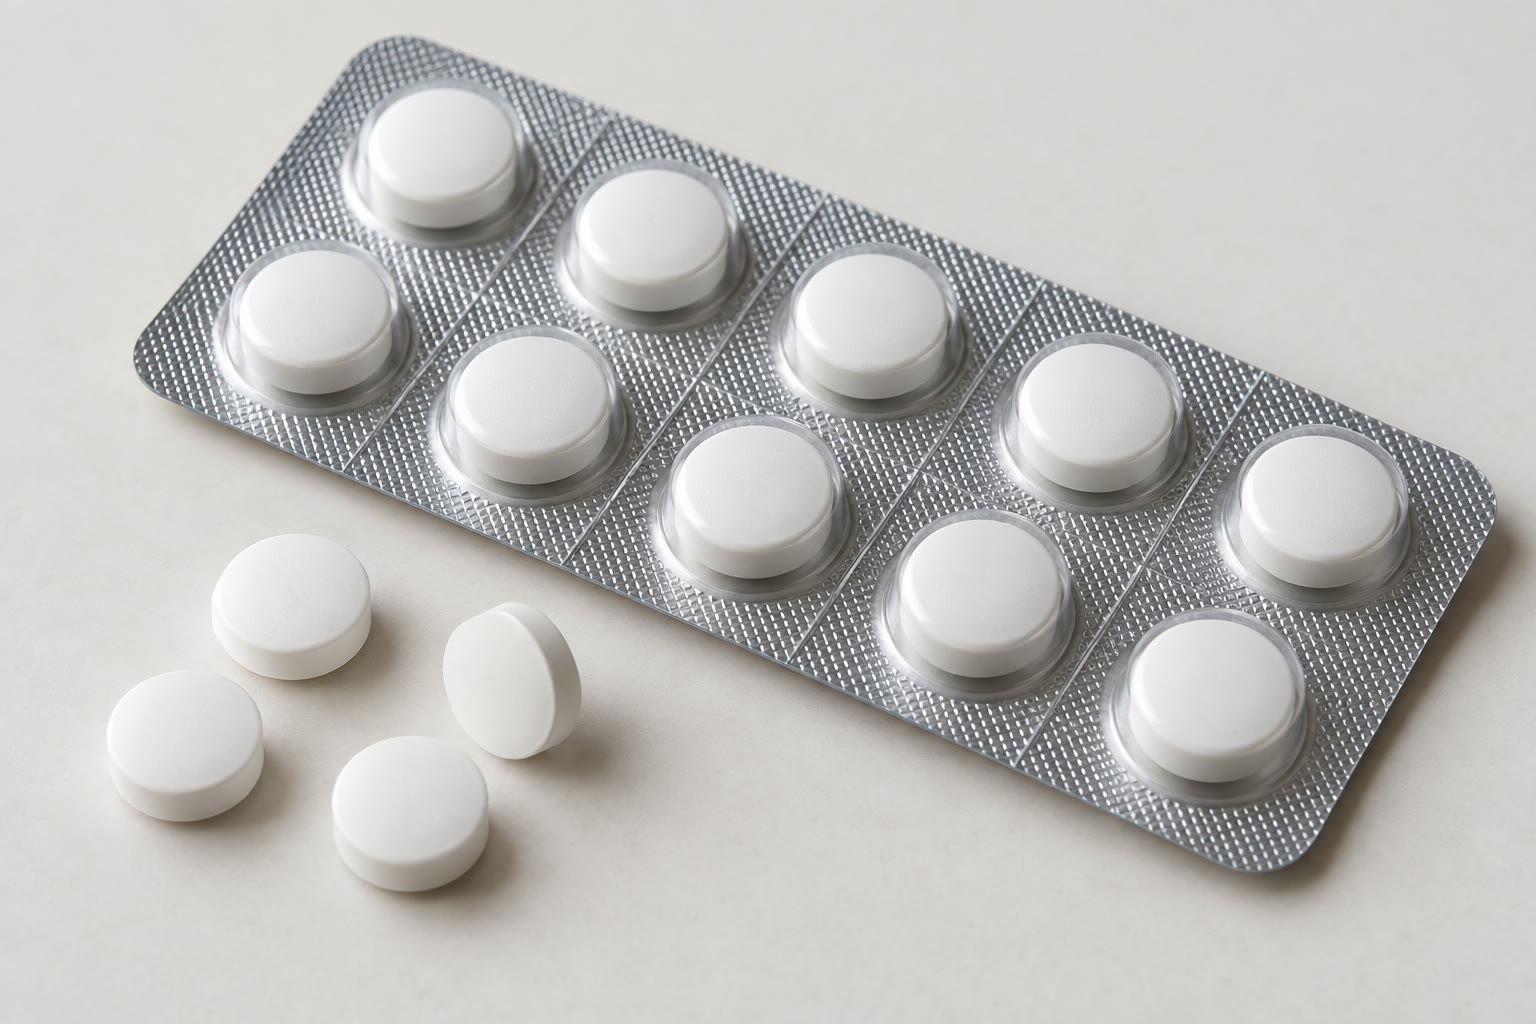
\includegraphics[width=0.45\linewidth]{images/book1/ai/g10-aspirin-tablets.jpg}

{\small Comprimidos de aspirina: cada um contém uma massa pesada da
\omterm{def:g6:pure-substances-and-mixtures:pure-substance}{substância pura}, \omterm{def:g2:mixing-and-dissolving:mix}{misturada} com um aglutinante.}
\end{omfigure}
\section{Exercícios}


\begin{exercise}[$\star$]\label{exo:g10:synthesis-yield:1}
Uma \omterm{def:g10:synthesis-yield:synthesis}{síntese} poderia dar no máximo \qty{5.0}{g} de produto; obtêm-se
\qty{4.2}{g} de produto puro e seco. Calcule o \omterm{def:g10:synthesis-yield:yield}{rendimento}.
\end{exercise}

\begin{exercise}[$\star$]\label{exo:g10:synthesis-yield:2}
Ponha em ordem estas etapas de uma \omterm{def:g10:synthesis-yield:synthesis}{síntese}: medição do ponto de fusão;
\omterm{def:g10:synthesis-yield:reflux}{aquecimento sob refluxo}; \omterm{def:g10:synthesis-yield:recrystallisation}{recristalização}; \omterm{def:g10:synthesis-yield:vacuum-filtration}{filtração a vácuo} do \omterm{def:g10:synthesis-yield:synthesis}{produto
bruto}; pesagem dos \omterm{def:g7:chemical-reactions:reactant}{reagentes}.
\end{exercise}

\begin{exercise}[$\star$]\label{exo:g10:synthesis-yield:3}
Numa montagem de refluxo, por que a água de resfriamento entra no
condensador por baixo? Por que o alto do condensador fica aberto?
\end{exercise}

\begin{exercise}[$\star$]\label{exo:g10:synthesis-yield:4}
Que duas propriedades um \omterm{def:g6:solutions-and-solubility:solute}{solvente} deve ter para recristalizar um
produto? Onde acabam as impurezas?
\end{exercise}

\begin{exercise}[$\star$]\label{exo:g10:synthesis-yield:5}
% ledger: mp:aspirin
Uma amostra de aspirina sintetizada funde entre \qty{124}{\celsius} e
\qty{130}{\celsius}. A aspirina pura funde a cerca de
\qty{135}{\celsius}. A amostra é pura? O que deve ser feito?
\end{exercise}

\begin{exercise}[$\star\star$]\label{exo:g10:synthesis-yield:6}
\qty{2.00}{g} de ácido salicílico reagem com anidrido etanoico em
excesso; obtêm-se \qty{2.03}{g} de aspirina pura e seca. Calcule a massa
máxima de aspirina e o \omterm{def:g10:synthesis-yield:yield}{rendimento}.
\end{exercise}

\begin{exercise}[$\star\star$]\label{exo:g10:synthesis-yield:7}
Uma aluna pesa a sua aspirina ainda úmida e encontra um \omterm{def:g10:synthesis-yield:yield}{rendimento} de
\qty{104}{\percent}. Explique. Pesar o \omterm{def:g10:synthesis-yield:synthesis}{produto bruto}, não purificado mas
seco, daria um \omterm{def:g10:synthesis-yield:yield}{rendimento} alto ou baixo demais em relação ao \omterm{def:g10:synthesis-yield:yield}{rendimento}
verdadeiro?
\end{exercise}

\begin{exercise}[$\star\star$]\label{exo:g10:synthesis-yield:8}
Dê duas vantagens de uma \omterm{def:g10:synthesis-yield:vacuum-filtration}{filtração a vácuo} sobre uma \omterm{def:g3:separating-mixtures:filter}{filtração} comum
num cone de papel, para recolher cristais.
\end{exercise}

\begin{exercise}[$\star\star$]\label{exo:g10:synthesis-yield:9}
Numa placa de cromatografia, a frente do \omterm{def:g6:solutions-and-solubility:solute}{solvente} percorreu
\qty{5.0}{cm}. A mancha de um produto sintetizado percorreu
\qty{3.1}{cm}, a da aspirina pura \qty{3.1}{cm}, a do ácido salicílico
\qty{2.2}{cm}. Calcule os três \omterm{def:g10:chemical-species:retention-factor}{fatores de retenção}. O que se pode
concluir sobre o produto?
\end{exercise}

\begin{exercise}[$\star\star$]\label{exo:g10:synthesis-yield:10}
A \omterm{def:g6:solutions-and-solubility:solubility}{solubilidade} de um produto em dois \omterm{def:g6:solutions-and-solubility:solute}{solventes} é:
\begin{center}
\begin{tabular}{lcc}
\hline
\omterm{def:g6:solutions-and-solubility:solute}{solvente} & a frio (\qty{20}{\celsius}) & a quente (perto da ebulição) \\
\hline
A & \qty{2}{g/L} & \qty{150}{g/L} \\
B & \qty{80}{g/L} & \qty{120}{g/L} \\
\hline
\end{tabular}
\end{center}
Que \omterm{def:g6:solutions-and-solubility:solute}{solvente} é melhor para uma \omterm{def:g10:synthesis-yield:recrystallisation}{recristalização}? Para \qty{3.0}{g} de
\omterm{def:g10:synthesis-yield:synthesis}{produto bruto}, mais ou menos que volume de \omterm{def:g6:solutions-and-solubility:solute}{solvente} quente é necessário,
e que massa, no máximo, continua dissolvida depois de frio?
\end{exercise}

\begin{exercise}[$\star\star$]\label{exo:g10:synthesis-yield:11}
Por que o balão de fundo redondo de uma montagem de refluxo nunca fica
mais do que meio cheio? Por que se acrescentam pedrinhas de ebulição?
\end{exercise}

\begin{exercise}[$\star\star\star$]\label{exo:g10:synthesis-yield:12}
Um remédio é produzido em duas etapas, de \omterm{def:g10:synthesis-yield:yield}{rendimentos}
\qty{80}{\percent} e \qty{70}{\percent}. Qual é o \omterm{def:g10:synthesis-yield:yield}{rendimento} global?
Qual seria ele para três etapas de \qty{90}{\percent} cada? Por que os
químicos procuram produzir os remédios no menor número possível de
etapas?
\end{exercise}

\begin{exercise}[$\star\star\star$]\label{exo:g10:synthesis-yield:13}
% ledger: sol:aspirin-25
A aspirina \omterm{def:g2:mixing-and-dissolving:dissolve}{se dissolve} na água até cerca de \qty{3.3}{g/L} a
\qty{25}{\celsius}. Cristais são lavados com \qty{50}{mL} de água a essa
temperatura. Que massa de aspirina pode ser perdida, no máximo? Por que
a água de lavagem é antes resfriada no gelo?
\end{exercise}

\begin{exercise}[$\star\star\star$]\label{exo:g10:synthesis-yield:14}
\qty{2.76}{g} de ácido salicílico são \omterm{def:g2:mixing-and-dissolving:mix}{misturados} com \qty{0.0500}{mol}
de anidrido etanoico. Depois da reação, acrescenta-se água, que destrói
o anidrido em excesso: \ce{C4H6O3 + H2O -> 2C2H4O2}.
\begin{enumerate}
  \item Preencha a \omterm{def:g10:reaction-progress-table:extent}{tabela de avanço} da \omterm{def:g10:synthesis-yield:synthesis}{síntese}; que quantidade de
        anidrido sobra?
  \item Que quantidade total de ácido etanoico está presente no fim?
\end{enumerate}
\end{exercise}

\begin{exercise}[$\star\star\star$]\label{exo:g10:synthesis-yield:15}
Uma fábrica precisa produzir \qty{1.00}{t} de aspirina, com um
\omterm{def:g10:synthesis-yield:yield}{rendimento} global de \qty{85}{\percent} a partir do ácido salicílico.
Que massa de ácido salicílico ela deve comprar?
\end{exercise}

\section{Problema: produzir aspirina}

\begin{problem}[{Problema de fim de semana --- de três gramas de ácido
salicílico a um frasco de aspirina pura: qual é o rendimento?}]
\label{pb:g10:synthesis-yield:1}
% ledger: rho:acetic-anhydride, mp:aspirin, mp:salicylic, sol:aspirin-25, aw:C, aw:H, aw:O
Uma turma produz aspirina. No balão: \qty{3.0}{g} de ácido salicílico e
\qty{6.0}{mL} de anidrido etanoico, de densidade \qty{1.08}{g/mL}, com
algumas gotas de ácido; a \omterm{def:g6:pure-substances-and-mixtures:mixture}{mistura} é aquecida sob refluxo. O \omterm{def:g10:synthesis-yield:synthesis}{produto
bruto} recolhido por \omterm{def:g10:synthesis-yield:vacuum-filtration}{filtração a vácuo} pesa \qty{3.6}{g} úmido e
\qty{3.3}{g} depois de seco. Depois da \omterm{def:g10:synthesis-yield:recrystallisation}{recristalização} e da secagem,
restam \qty{2.7}{g} de cristais brancos.

\medskip
\noindent\textbf{Parte I --- A reação.}
\begin{enumerate}
  \item Verifique que a equação
        \ce{C7H6O3 + C4H6O3 -> C9H8O4 + C2H4O2} está balanceada.
  \item Calcule as \omterm{def:g10:the-mole:molar-mass}{massas molares} do ácido salicílico, do anidrido
        etanoico, da aspirina e do ácido etanoico.
  \item Dê o nome dos \omterm{def:g7:chemical-reactions:reactant}{reagentes}, do produto desejado e do subproduto.
  \item Por que a \omterm{def:g6:pure-substances-and-mixtures:mixture}{mistura} é aquecida sob refluxo, e não num frasco
        aberto?
\end{enumerate}

\medskip
\noindent\textbf{Parte II --- A massa máxima.}
\begin{enumerate}[resume]
  \item Calcule a quantidade inicial de ácido salicílico.
  \item Calcule a massa, e depois a quantidade, de anidrido etanoico.
  \item Preencha a \omterm{def:g10:reaction-progress-table:extent}{tabela de avanço}. Que \omterm{def:g7:chemical-reactions:reactant}{reagente} é limitante? Dê
        $x_{\max}$.
  \item Deduza a massa máxima de aspirina.
  \item Por que é o anidrido, e não o ácido salicílico, que é colocado
        em excesso?
\end{enumerate}

\medskip
\noindent\textbf{Parte III --- Isolar e purificar.}
\begin{enumerate}[resume]
  \item Por que a massa úmida, \qty{3.6}{g}, não pode ser usada para
        calcular um \omterm{def:g10:synthesis-yield:yield}{rendimento}?
  \item Calcule o \omterm{def:g10:synthesis-yield:yield}{rendimento} em \omterm{def:g10:synthesis-yield:synthesis}{produto bruto} seco.
  \item Por que a \omterm{def:g10:synthesis-yield:recrystallisation}{recristalização} diminui a massa?
  \item Os cristais foram lavados com \qty{30}{mL} de água a
        \qty{25}{\celsius}, temperatura em que a aspirina \omterm{def:g2:mixing-and-dissolving:dissolve}{se dissolve} até
        cerca de \qty{3.3}{g/L}. Que massa poderia ser perdida assim, no
        máximo?
  \item Calcule o \omterm{def:g10:synthesis-yield:yield}{rendimento} em produto puro.
\end{enumerate}

\medskip
\noindent\textbf{Parte IV --- Verificar o produto.}
\begin{enumerate}[resume]
  \item Os cristais recristalizados fundem de uma vez a
        \qty{135}{\celsius}. O que isso mostra?
  \item O \omterm{def:g10:synthesis-yield:synthesis}{produto bruto} fundia entre \qty{120}{\celsius} e
        \qty{131}{\celsius}. O que isso mostra?
  \item Numa placa de cromatografia, o \omterm{def:g10:synthesis-yield:synthesis}{produto bruto} dá duas manchas,
        uma na altura da aspirina pura e outra na altura do ácido
        salicílico; o produto recristalizado dá uma única mancha, na
        altura da aspirina. Conclua.
  \item A mancha do produto recristalizado percorreu \qty{3.1}{cm} e a
        frente do \omterm{def:g6:solutions-and-solubility:solute}{solvente} \qty{5.0}{cm}. Calcule o seu \omterm{def:g10:chemical-species:retention-factor}{fator de
        retenção}.
  \item Entre a reação e a \omterm{def:g10:synthesis-yield:recrystallisation}{recristalização}, que parte do trabalho perdeu
        mais aspirina?
  \item Dê a resposta final: qual é o \omterm{def:g10:synthesis-yield:yield}{rendimento} da \omterm{def:g10:synthesis-yield:synthesis}{síntese}?
\end{enumerate}
\end{problem}
